\documentclass[1p]{elsarticle_modified}
%\bibliographystyle{elsarticle-num}

%\usepackage[colorlinks]{hyperref}
%\usepackage{abbrmath_seonhwa} %\Abb, \Ascr, \Acal ,\Abf, \Afrak
\usepackage{amsfonts}
\usepackage{amssymb}
\usepackage{amsmath}
\usepackage{amsthm}
\usepackage{scalefnt}
\usepackage{amsbsy}
\usepackage{kotex}
\usepackage{caption}
\usepackage{subfig}
\usepackage{color}
\usepackage{graphicx}
\usepackage{xcolor} %% white, black, red, green, blue, cyan, magenta, yellow
\usepackage{float}
\usepackage{setspace}
\usepackage{hyperref}

\usepackage{tikz}
\usetikzlibrary{arrows}

\usepackage{multirow}
\usepackage{array} % fixed length table
\usepackage{hhline}

%%%%%%%%%%%%%%%%%%%%%
\makeatletter
\renewcommand*\env@matrix[1][\arraystretch]{%
	\edef\arraystretch{#1}%
	\hskip -\arraycolsep
	\let\@ifnextchar\new@ifnextchar
	\array{*\c@MaxMatrixCols c}}
\makeatother %https://tex.stackexchange.com/questions/14071/how-can-i-increase-the-line-spacing-in-a-matrix
%%%%%%%%%%%%%%%

\usepackage[normalem]{ulem}

\newcommand{\msout}[1]{\ifmmode\text{\sout{\ensuremath{#1}}}\else\sout{#1}\fi}
%SOURCE: \msout is \stkout macro in https://tex.stackexchange.com/questions/20609/strikeout-in-math-mode

\newcommand{\cancel}[1]{
	\ifmmode
	{\color{red}\msout{#1}}
	\else
	{\color{red}\sout{#1}}
	\fi
}

\newcommand{\add}[1]{
	{\color{blue}\uwave{#1}}
}

\newcommand{\replace}[2]{
	\ifmmode
	{\color{red}\msout{#1}}{\color{blue}\uwave{#2}}
	\else
	{\color{red}\sout{#1}}{\color{blue}\uwave{#2}}
	\fi
}

\newcommand{\Sol}{\mathcal{S}} %segment
\newcommand{\D}{D} %diagram
\newcommand{\A}{\mathcal{A}} %arc


%%%%%%%%%%%%%%%%%%%%%%%%%%%%%5 test

\def\sl{\operatorname{\textup{SL}}(2,\Cbb)}
\def\psl{\operatorname{\textup{PSL}}(2,\Cbb)}
\def\quan{\mkern 1mu \triangleright \mkern 1mu}

\theoremstyle{definition}
\newtheorem{thm}{Theorem}[section]
\newtheorem{prop}[thm]{Proposition}
\newtheorem{lem}[thm]{Lemma}
\newtheorem{ques}[thm]{Question}
\newtheorem{cor}[thm]{Corollary}
\newtheorem{defn}[thm]{Definition}
\newtheorem{exam}[thm]{Example}
\newtheorem{rmk}[thm]{Remark}
\newtheorem{alg}[thm]{Algorithm}

\newcommand{\I}{\sqrt{-1}}
\begin{document}

%\begin{frontmatter}
%
%\title{Boundary parabolic representations of knots up to 8 crossings}
%
%%% Group authors per affiliation:
%\author{Yunhi Cho} 
%\address{Department of Mathematics, University of Seoul, Seoul, Korea}
%\ead{yhcho@uos.ac.kr}
%
%
%\author{Seonhwa Kim} %\fnref{s_kim}}
%\address{Center for Geometry and Physics, Institute for Basic Science, Pohang, 37673, Korea}
%\ead{ryeona17@ibs.re.kr}
%
%\author{Hyuk Kim}
%\address{Department of Mathematical Sciences, Seoul National University, Seoul 08826, Korea}
%\ead{hyukkim@snu.ac.kr}
%
%\author{Seokbeom Yoon}
%\address{Department of Mathematical Sciences, Seoul National University, Seoul, 08826,  Korea}
%\ead{sbyoon15@snu.ac.kr}
%
%\begin{abstract}
%We find all boundary parabolic representation of knots up to 8 crossings.
%
%\end{abstract}
%\begin{keyword}
%    \MSC[2010] 57M25 
%\end{keyword}
%
%\end{frontmatter}

%\linenumbers
%\tableofcontents
%
\newcommand\colored[1]{\textcolor{white}{\rule[-0.35ex]{0.8em}{1.4ex}}\kern-0.8em\color{red} #1}%
%\newcommand\colored[1]{\textcolor{white}{ #1}\kern-2.17ex	\textcolor{white}{ #1}\kern-1.81ex	\textcolor{white}{ #1}\kern-2.15ex\color{red}#1	}

{\Large $\underline{11n_{45}~(K11n_{45})}$}

\setlength{\tabcolsep}{10pt}
\renewcommand{\arraystretch}{1.6}
\vspace{1cm}\begin{tabular}{m{100pt}>{\centering\arraybackslash}m{274pt}}
\multirow{5}{120pt}{
	\centering
	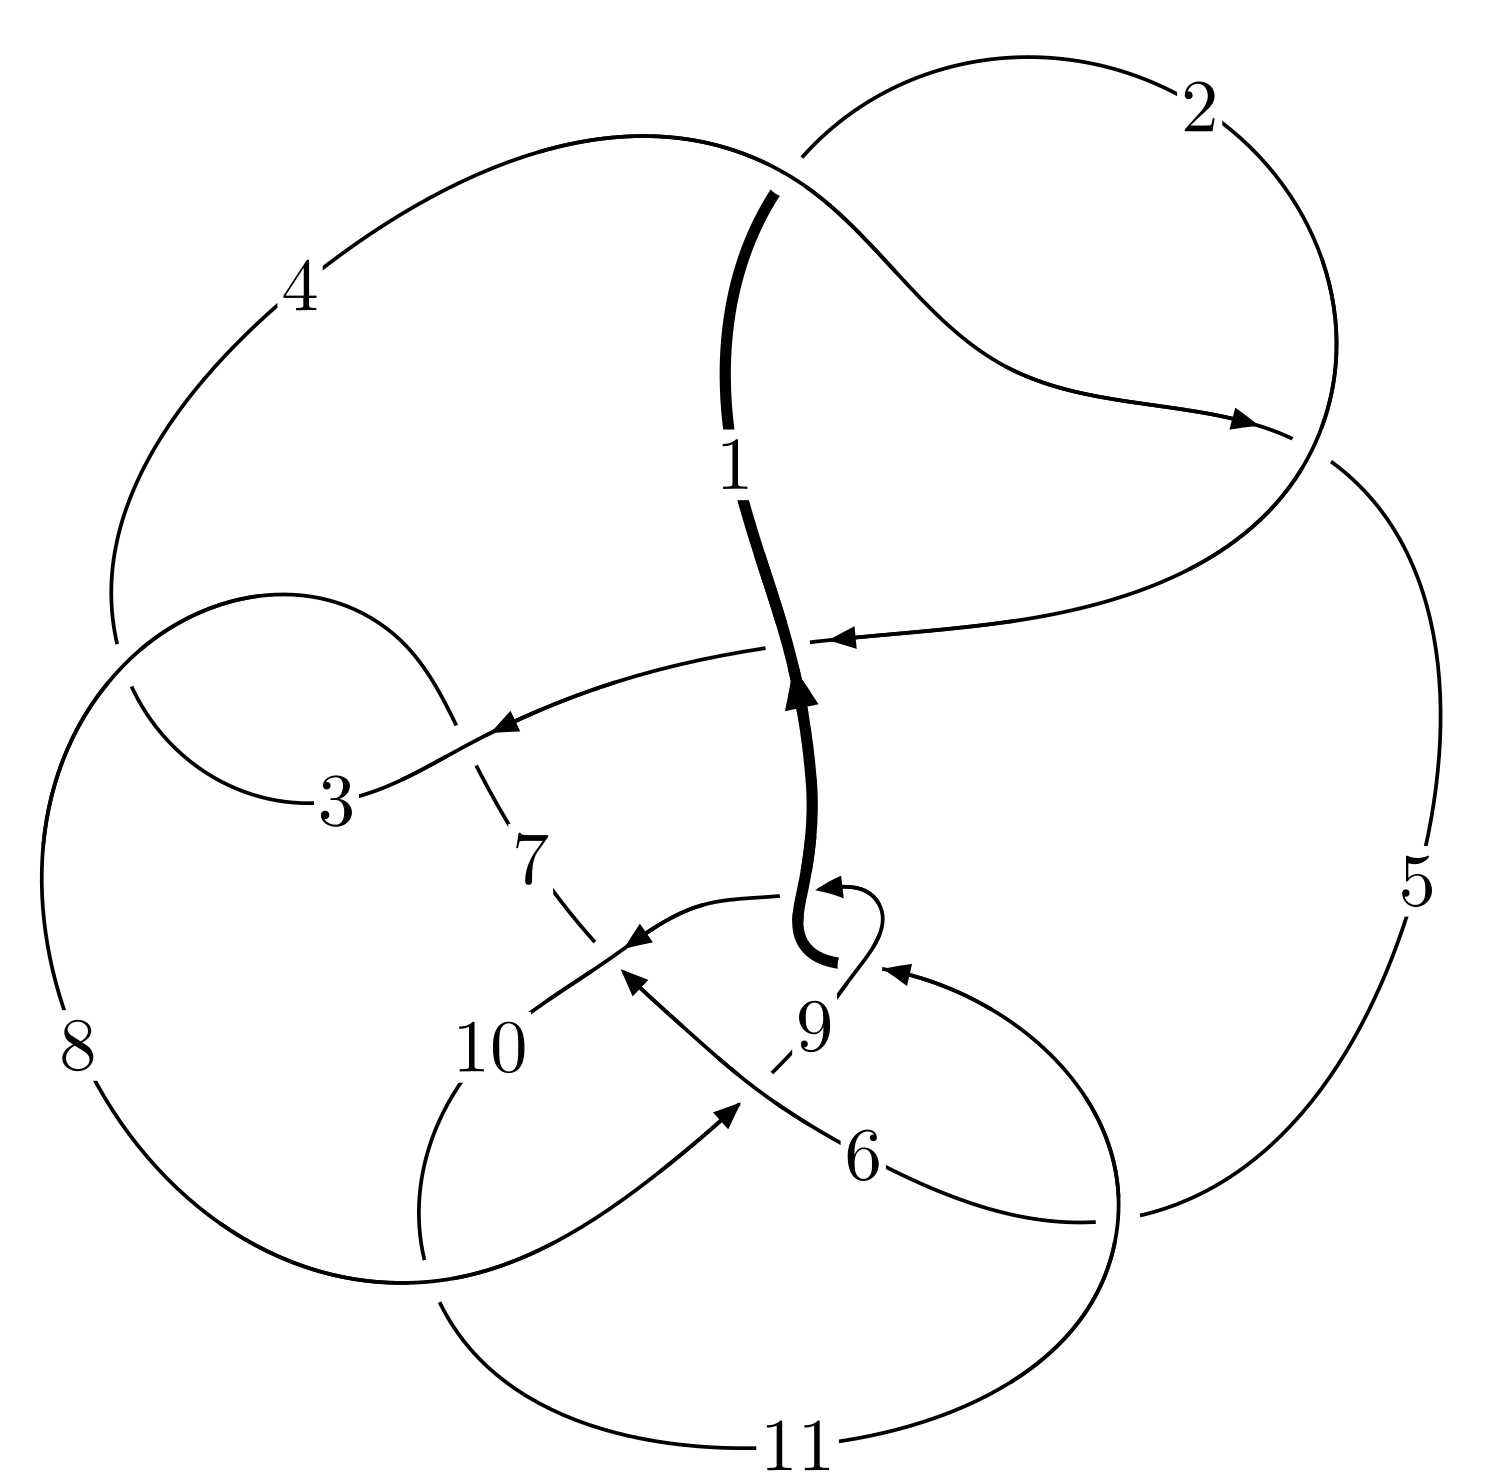
\includegraphics[width=112pt]{../../../GIT/diagram.site/Diagrams/png/661_11n_45.png}\\
\ \ \ A knot diagram\footnotemark}&
\allowdisplaybreaks
\textbf{Linearized knot diagam} \\
\cline{2-2}
 &
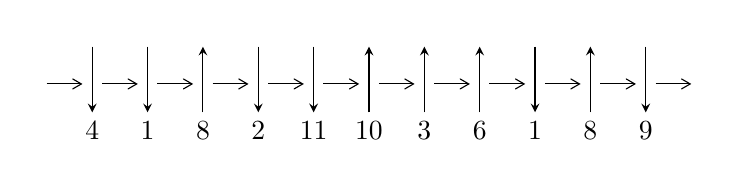
\begin{tikzpicture}[x=20pt, y=17pt]
	% nodes
	\node (C0) at (0, 0) {};
	\node (C1) at (1, 0) {};
	\node (C1U) at (1, +1) {};
	\node (C1D) at (1, -1) {4};

	\node (C2) at (2, 0) {};
	\node (C2U) at (2, +1) {};
	\node (C2D) at (2, -1) {1};

	\node (C3) at (3, 0) {};
	\node (C3U) at (3, +1) {};
	\node (C3D) at (3, -1) {8};

	\node (C4) at (4, 0) {};
	\node (C4U) at (4, +1) {};
	\node (C4D) at (4, -1) {2};

	\node (C5) at (5, 0) {};
	\node (C5U) at (5, +1) {};
	\node (C5D) at (5, -1) {11};

	\node (C6) at (6, 0) {};
	\node (C6U) at (6, +1) {};
	\node (C6D) at (6, -1) {10};

	\node (C7) at (7, 0) {};
	\node (C7U) at (7, +1) {};
	\node (C7D) at (7, -1) {3};

	\node (C8) at (8, 0) {};
	\node (C8U) at (8, +1) {};
	\node (C8D) at (8, -1) {6};

	\node (C9) at (9, 0) {};
	\node (C9U) at (9, +1) {};
	\node (C9D) at (9, -1) {1};

	\node (C10) at (10, 0) {};
	\node (C10U) at (10, +1) {};
	\node (C10D) at (10, -1) {8};

	\node (C11) at (11, 0) {};
	\node (C11U) at (11, +1) {};
	\node (C11D) at (11, -1) {9};
	\node (C12) at (12, 0) {};

	% arrows
	\draw[->,>={angle 60}]
	(C0) edge (C1) (C1) edge (C2) (C2) edge (C3) (C3) edge (C4) (C4) edge (C5) (C5) edge (C6) (C6) edge (C7) (C7) edge (C8) (C8) edge (C9) (C9) edge (C10) (C10) edge (C11) (C11) edge (C12) ;	\draw[->,>=stealth]
	(C1U) edge (C1D) (C2U) edge (C2D) (C3D) edge (C3U) (C4U) edge (C4D) (C5U) edge (C5D) (C6D) edge (C6U) (C7D) edge (C7U) (C8D) edge (C8U) (C9U) edge (C9D) (C10D) edge (C10U) (C11U) edge (C11D) ;
	\end{tikzpicture} \\
\hhline{~~} \\& 
\textbf{Solving Sequence} \\ \cline{2-2} 
 &
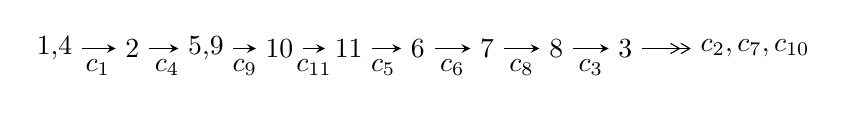
\begin{tikzpicture}[x=25pt, y=7pt]
	% node
	\node (A0) at (-1/8, 0) {1,4};
	\node (A1) at (1, 0) {2};
	\node (A2) at (33/16, 0) {5,9};
	\node (A3) at (25/8, 0) {10};
	\node (A4) at (33/8, 0) {11};
	\node (A5) at (41/8, 0) {6};
	\node (A6) at (49/8, 0) {7};
	\node (A7) at (57/8, 0) {8};
	\node (A8) at (65/8, 0) {3};
	\node (C1) at (1/2, -1) {$c_{1}$};
	\node (C2) at (3/2, -1) {$c_{4}$};
	\node (C3) at (21/8, -1) {$c_{9}$};
	\node (C4) at (29/8, -1) {$c_{11}$};
	\node (C5) at (37/8, -1) {$c_{5}$};
	\node (C6) at (45/8, -1) {$c_{6}$};
	\node (C7) at (53/8, -1) {$c_{8}$};
	\node (C8) at (61/8, -1) {$c_{3}$};
	\node (A9) at (10, 0) {$c_{2},c_{7},c_{10}$};

	% edge
	\draw[->,>=stealth]	
	(A0) edge (A1) (A1) edge (A2) (A2) edge (A3) (A3) edge (A4) (A4) edge (A5) (A5) edge (A6) (A6) edge (A7) (A7) edge (A8) ;
	\draw[->>,>={angle 60}]	
	(A8) edge (A9);
\end{tikzpicture} \\ 

\end{tabular} \\

\footnotetext{
The image of knot diagram is generated by the software ``\textbf{Draw programme}" developed by Andrew Bartholomew(\url{http://www.layer8.co.uk/maths/draw/index.htm\#Running-draw}), where we modified some parts for our purpose(\url{https://github.com/CATsTAILs/LinksPainter}).
}\phantom \\ \newline 
\centering \textbf{Ideals for irreducible components\footnotemark of $X_{\text{par}}$} 
 
\begin{align*}
I^u_{1}&=\langle 
b+u,\;a- u-2,\;u^{12}+5 u^{11}+9 u^{10}-21 u^8-22 u^7+10 u^6+26 u^5+4 u^4-11 u^3-3 u^2+2 u+1\rangle \\
I^u_{2}&=\langle 
b+1,\;u^5+u^4- u^3-2 u^2+a+1,\;u^6+u^5- u^4-2 u^3+u+1\rangle \\
I^u_{3}&=\langle 
b^6- b^5- b^4+2 b^3- b+1,\;a-1,\;u-1\rangle \\
I^u_{4}&=\langle 
- u^{11}-2 u^{10}-6 u^9- u^8-7 u^7+15 u^6-14 u^5+28 u^4-50 u^3+41 u^2+32 b-66 u+31,\\
\phantom{I^u_{4}}&\phantom{= \langle  }u^{11}+3 u^{10}+8 u^9+7 u^8+8 u^7-8 u^6- u^5-14 u^4+22 u^3+9 u^2+a+25 u+3,\\
\phantom{I^u_{4}}&\phantom{= \langle  }u^{12}+3 u^{11}+8 u^{10}+7 u^9+8 u^8-8 u^7- u^6-14 u^5+22 u^4+9 u^3+25 u^2+3 u+1\rangle \\
\\
\end{align*}
\raggedright * 4 irreducible components of $\dim_{\mathbb{C}}=0$, with total 36 representations.\\
\footnotetext{All coefficients of polynomials are rational numbers. But the coefficients are sometimes approximated in decimal forms when there is not enough margin.}
\newpage
\renewcommand{\arraystretch}{1}
\centering \section*{I. $I^u_{1}= \langle b+u,\;a- u-2,\;u^{12}+5 u^{11}+\cdots+2 u+1 \rangle$}
\flushleft \textbf{(i) Arc colorings}\\
\begin{tabular}{m{7pt} m{180pt} m{7pt} m{180pt} }
\flushright $a_{1}=$&$\begin{pmatrix}1\\0\end{pmatrix}$ \\
\flushright $a_{4}=$&$\begin{pmatrix}0\\u\end{pmatrix}$ \\
\flushright $a_{2}=$&$\begin{pmatrix}1\\u^2\end{pmatrix}$ \\
\flushright $a_{5}=$&$\begin{pmatrix}- u\\- u^3+u\end{pmatrix}$ \\
\flushright $a_{9}=$&$\begin{pmatrix}u+2\\- u\end{pmatrix}$ \\
\flushright $a_{10}=$&$\begin{pmatrix}2 u+2\\- u\end{pmatrix}$ \\
\flushright $a_{11}=$&$\begin{pmatrix}u^2+2 u+1\\- u^2\end{pmatrix}$ \\
\flushright $a_{6}=$&$\begin{pmatrix}u^7+4 u^6+6 u^5+2 u^4-4 u^3-4 u^2-2 u\\- u^7-2 u^6- u^5+2 u^4+u\end{pmatrix}$ \\
\flushright $a_{7}=$&$\begin{pmatrix}-2 u^9-6 u^8-3 u^7+12 u^6+14 u^5-6 u^4-12 u^3+2 u\\u^9+2 u^8- u^7-6 u^6- u^5+6 u^4-2 u^2+u\end{pmatrix}$ \\
\flushright $a_{8}=$&$\begin{pmatrix}u^{10}+4 u^9+5 u^8-4 u^7-14 u^6-6 u^5+11 u^4+8 u^3-3 u^2-2 u+1\\- u^{11}-5 u^{10}+\cdots-2 u-1\end{pmatrix}$ \\
\flushright $a_{3}=$&$\begin{pmatrix}- u^2+1\\u^2\end{pmatrix}$\\ \flushright $a_{3}=$&$\begin{pmatrix}- u^2+1\\u^2\end{pmatrix}$\\&\end{tabular}
\flushleft \textbf{(ii) Obstruction class $= -1$}\\~\\
\flushleft \textbf{(iii) Cusp Shapes $= -4 u^{11}-16 u^{10}-24 u^9+24 u^7-32 u^5+16 u^4+36 u^3-16 u+2$}\\~\\
\newpage\renewcommand{\arraystretch}{1}
\flushleft \textbf{(iv) u-Polynomials at the component}\newline \\
\begin{tabular}{m{50pt}|m{274pt}}
Crossings & \hspace{64pt}u-Polynomials at each crossing \\
\hline $$\begin{aligned}c_{1},c_{4},c_{9}\\c_{11}\end{aligned}$$&$\begin{aligned}
&u^{12}-5 u^{11}+\cdots-2 u+1
\end{aligned}$\\
\hline $$\begin{aligned}c_{2}\end{aligned}$$&$\begin{aligned}
&u^{12}+7 u^{11}+\cdots+10 u+1
\end{aligned}$\\
\hline $$\begin{aligned}c_{3},c_{7},c_{10}\end{aligned}$$&$\begin{aligned}
&u^{12}+u^{11}+\cdots+2 u+1
\end{aligned}$\\
\hline $$\begin{aligned}c_{5}\end{aligned}$$&$\begin{aligned}
&u^{12}-3 u^{11}+\cdots-14 u+4
\end{aligned}$\\
\hline $$\begin{aligned}c_{6}\end{aligned}$$&$\begin{aligned}
&u^{12}- u^{11}+\cdots+44 u+23
\end{aligned}$\\
\hline $$\begin{aligned}c_{8}\end{aligned}$$&$\begin{aligned}
&u^{12}+u^{11}+u^{10}+5 u^8-4 u^6-8 u^5+6 u^4+3 u^3+3 u^2+1
\end{aligned}$\\
\hline
\end{tabular}\\~\\
\newpage\renewcommand{\arraystretch}{1}
\flushleft \textbf{(v) Riley Polynomials at the component}\newline \\
\begin{tabular}{m{50pt}|m{274pt}}
Crossings & \hspace{64pt}Riley Polynomials at each crossing \\
\hline $$\begin{aligned}c_{1},c_{4},c_{9}\\c_{11}\end{aligned}$$&$\begin{aligned}
&y^{12}-7 y^{11}+\cdots-10 y+1
\end{aligned}$\\
\hline $$\begin{aligned}c_{2}\end{aligned}$$&$\begin{aligned}
&y^{12}+29 y^{11}+\cdots+22 y+1
\end{aligned}$\\
\hline $$\begin{aligned}c_{3},c_{7},c_{10}\end{aligned}$$&$\begin{aligned}
&y^{12}-15 y^{11}+\cdots-2 y+1
\end{aligned}$\\
\hline $$\begin{aligned}c_{5}\end{aligned}$$&$\begin{aligned}
&y^{12}+5 y^{11}+\cdots+68 y+16
\end{aligned}$\\
\hline $$\begin{aligned}c_{6}\end{aligned}$$&$\begin{aligned}
&y^{12}-23 y^{11}+\cdots-4098 y+529
\end{aligned}$\\
\hline $$\begin{aligned}c_{8}\end{aligned}$$&$\begin{aligned}
&y^{12}+y^{11}+\cdots+6 y+1
\end{aligned}$\\
\hline
\end{tabular}\\~\\
\newpage\flushleft \textbf{(vi) Complex Volumes and Cusp Shapes}
$$\begin{array}{c|c|c}  
\text{Solutions to }I^u_{1}& \I (\text{vol} + \sqrt{-1}CS) & \text{Cusp shape}\\
 \hline 
\begin{aligned}
u &= \phantom{-}1.017000 + 0.101771 I \\
a &= \phantom{-}3.01700 + 0.10177 I \\
b &= -1.017000 - 0.101771 I\end{aligned}
 & -3.52730 - 0.57280 I & -2.7091 - 26.6989 I \\ \hline\begin{aligned}
u &= \phantom{-}1.017000 - 0.101771 I \\
a &= \phantom{-}3.01700 - 0.10177 I \\
b &= -1.017000 + 0.101771 I\end{aligned}
 & -3.52730 + 0.57280 I & -2.7091 + 26.6989 I \\ \hline\begin{aligned}
u &= -0.997809 + 0.382742 I \\
a &= \phantom{-}1.002190 + 0.382742 I \\
b &= \phantom{-}0.997809 - 0.382742 I\end{aligned}
 & -1.70690 + 6.65526 I & -0.69156 - 12.28500 I \\ \hline\begin{aligned}
u &= -0.997809 - 0.382742 I \\
a &= \phantom{-}1.002190 - 0.382742 I \\
b &= \phantom{-}0.997809 + 0.382742 I\end{aligned}
 & -1.70690 - 6.65526 I & -0.69156 + 12.28500 I \\ \hline\begin{aligned}
u &= \phantom{-}0.568808 + 0.252332 I \\
a &= \phantom{-}2.56881 + 0.25233 I \\
b &= -0.568808 - 0.252332 I\end{aligned}
 & -1.61529 - 1.35793 I & -3.64822 + 4.51645 I \\ \hline\begin{aligned}
u &= \phantom{-}0.568808 - 0.252332 I \\
a &= \phantom{-}2.56881 - 0.25233 I \\
b &= -0.568808 + 0.252332 I\end{aligned}
 & -1.61529 + 1.35793 I & -3.64822 - 4.51645 I \\ \hline\begin{aligned}
u &= -0.417930 + 0.278210 I \\
a &= \phantom{-}1.58207 + 0.27821 I \\
b &= \phantom{-}0.417930 - 0.278210 I\end{aligned}
 & \phantom{-}1.46216 - 0.16286 I & \phantom{-}7.96188 - 1.03516 I \\ \hline\begin{aligned}
u &= -0.417930 - 0.278210 I \\
a &= \phantom{-}1.58207 - 0.27821 I \\
b &= \phantom{-}0.417930 + 0.278210 I\end{aligned}
 & \phantom{-}1.46216 + 0.16286 I & \phantom{-}7.96188 + 1.03516 I \\ \hline\begin{aligned}
u &= -1.29679 + 1.06566 I \\
a &= \phantom{-}0.703205 + 1.065660 I \\
b &= \phantom{-}1.29679 - 1.06566 I\end{aligned}
 & \phantom{-}12.72390 + 5.46645 I & -0.22295 - 2.11548 I \\ \hline\begin{aligned}
u &= -1.29679 - 1.06566 I \\
a &= \phantom{-}0.703205 - 1.065660 I \\
b &= \phantom{-}1.29679 + 1.06566 I\end{aligned}
 & \phantom{-}12.72390 - 5.46645 I & -0.22295 + 2.11548 I\\
 \hline 
 \end{array}$$\newpage$$\begin{array}{c|c|c}  
\text{Solutions to }I^u_{1}& \I (\text{vol} + \sqrt{-1}CS) & \text{Cusp shape}\\
 \hline 
\begin{aligned}
u &= -1.37328 + 1.07803 I \\
a &= \phantom{-}0.626724 + 1.078030 I \\
b &= \phantom{-}1.37328 - 1.07803 I\end{aligned}
 & \phantom{-}12.4026 + 12.7511 I & -0.69002 - 5.94531 I \\ \hline\begin{aligned}
u &= -1.37328 - 1.07803 I \\
a &= \phantom{-}0.626724 - 1.078030 I \\
b &= \phantom{-}1.37328 + 1.07803 I\end{aligned}
 & \phantom{-}12.4026 - 12.7511 I & -0.69002 + 5.94531 I\\
 \hline 
 \end{array}$$\newpage\newpage\renewcommand{\arraystretch}{1}
\centering \section*{II. $I^u_{2}= \langle b+1,\;u^5+u^4- u^3-2 u^2+a+1,\;u^6+u^5- u^4-2 u^3+u+1 \rangle$}
\flushleft \textbf{(i) Arc colorings}\\
\begin{tabular}{m{7pt} m{180pt} m{7pt} m{180pt} }
\flushright $a_{1}=$&$\begin{pmatrix}1\\0\end{pmatrix}$ \\
\flushright $a_{4}=$&$\begin{pmatrix}0\\u\end{pmatrix}$ \\
\flushright $a_{2}=$&$\begin{pmatrix}1\\u^2\end{pmatrix}$ \\
\flushright $a_{5}=$&$\begin{pmatrix}- u\\- u^3+u\end{pmatrix}$ \\
\flushright $a_{9}=$&$\begin{pmatrix}- u^5- u^4+u^3+2 u^2-1\\-1\end{pmatrix}$ \\
\flushright $a_{10}=$&$\begin{pmatrix}- u^5- u^4+u^3+2 u^2\\-1\end{pmatrix}$ \\
\flushright $a_{11}=$&$\begin{pmatrix}- u^5- u^4+u^3+2 u^2\\-1\end{pmatrix}$ \\
\flushright $a_{6}=$&$\begin{pmatrix}u^5+u^4\\-2 u^3- u^2+u+1\end{pmatrix}$ \\
\flushright $a_{7}=$&$\begin{pmatrix}- u\\- u^3+u\end{pmatrix}$ \\
\flushright $a_{8}=$&$\begin{pmatrix}- u^4+u^2-1\\u^5+u^4-2 u^3- u^2+u+1\end{pmatrix}$ \\
\flushright $a_{3}=$&$\begin{pmatrix}- u^2+1\\u^2\end{pmatrix}$\\ \flushright $a_{3}=$&$\begin{pmatrix}- u^2+1\\u^2\end{pmatrix}$\\&\end{tabular}
\flushleft \textbf{(ii) Obstruction class $= 1$}\\~\\
\flushleft \textbf{(iii) Cusp Shapes $= 3 u^5+7 u^4+u^3-6 u^2-5 u-1$}\\~\\
\newpage\renewcommand{\arraystretch}{1}
\flushleft \textbf{(iv) u-Polynomials at the component}\newline \\
\begin{tabular}{m{50pt}|m{274pt}}
Crossings & \hspace{64pt}u-Polynomials at each crossing \\
\hline $$\begin{aligned}c_{1},c_{7}\end{aligned}$$&$\begin{aligned}
&u^6+u^5- u^4-2 u^3+u+1
\end{aligned}$\\
\hline $$\begin{aligned}c_{2}\end{aligned}$$&$\begin{aligned}
&u^6+3 u^5+5 u^4+4 u^3+2 u^2+u+1
\end{aligned}$\\
\hline $$\begin{aligned}c_{3},c_{4}\end{aligned}$$&$\begin{aligned}
&u^6- u^5- u^4+2 u^3- u+1
\end{aligned}$\\
\hline $$\begin{aligned}c_{5},c_{6}\end{aligned}$$&$\begin{aligned}
&u^6+u^5+2 u^4+4 u^3+5 u^2+3 u+1
\end{aligned}$\\
\hline $$\begin{aligned}c_{8}\end{aligned}$$&$\begin{aligned}
&u^6-3 u^5+5 u^4-4 u^3+2 u^2- u+1
\end{aligned}$\\
\hline $$\begin{aligned}c_{9}\end{aligned}$$&$\begin{aligned}
&(u-1)^6
\end{aligned}$\\
\hline $$\begin{aligned}c_{10}\end{aligned}$$&$\begin{aligned}
&u^6
\end{aligned}$\\
\hline $$\begin{aligned}c_{11}\end{aligned}$$&$\begin{aligned}
&(u+1)^6
\end{aligned}$\\
\hline
\end{tabular}\\~\\
\newpage\renewcommand{\arraystretch}{1}
\flushleft \textbf{(v) Riley Polynomials at the component}\newline \\
\begin{tabular}{m{50pt}|m{274pt}}
Crossings & \hspace{64pt}Riley Polynomials at each crossing \\
\hline $$\begin{aligned}c_{1},c_{3},c_{4}\\c_{7}\end{aligned}$$&$\begin{aligned}
&y^6-3 y^5+5 y^4-4 y^3+2 y^2- y+1
\end{aligned}$\\
\hline $$\begin{aligned}c_{2},c_{8}\end{aligned}$$&$\begin{aligned}
&y^6+y^5+5 y^4+6 y^2+3 y+1
\end{aligned}$\\
\hline $$\begin{aligned}c_{5},c_{6}\end{aligned}$$&$\begin{aligned}
&y^6+3 y^5+6 y^4+5 y^2+y+1
\end{aligned}$\\
\hline $$\begin{aligned}c_{9},c_{11}\end{aligned}$$&$\begin{aligned}
&(y-1)^6
\end{aligned}$\\
\hline $$\begin{aligned}c_{10}\end{aligned}$$&$\begin{aligned}
&y^6
\end{aligned}$\\
\hline
\end{tabular}\\~\\
\newpage\flushleft \textbf{(vi) Complex Volumes and Cusp Shapes}
$$\begin{array}{c|c|c}  
\text{Solutions to }I^u_{2}& \I (\text{vol} + \sqrt{-1}CS) & \text{Cusp shape}\\
 \hline 
\begin{aligned}
u &= \phantom{-}1.002190 + 0.295542 I \\
a &= \phantom{-}0.917982 - 0.270708 I \\
b &= -1.00000\phantom{ +0.000000I}\end{aligned}
 & -3.53554 - 0.92430 I & -6.82874 + 7.13914 I \\ \hline\begin{aligned}
u &= \phantom{-}1.002190 - 0.295542 I \\
a &= \phantom{-}0.917982 + 0.270708 I \\
b &= -1.00000\phantom{ +0.000000I}\end{aligned}
 & -3.53554 + 0.92430 I & -6.82874 - 7.13914 I \\ \hline\begin{aligned}
u &= -0.428243 + 0.664531 I \\
a &= -0.685196 - 1.063260 I \\
b &= -1.00000\phantom{ +0.000000I}\end{aligned}
 & \phantom{-}0.245672 - 0.924305 I & \phantom{-}1.12292 + 1.33143 I \\ \hline\begin{aligned}
u &= -0.428243 - 0.664531 I \\
a &= -0.685196 + 1.063260 I \\
b &= -1.00000\phantom{ +0.000000I}\end{aligned}
 & \phantom{-}0.245672 + 0.924305 I & \phantom{-}1.12292 - 1.33143 I \\ \hline\begin{aligned}
u &= -1.073950 + 0.558752 I \\
a &= -0.732786 - 0.381252 I \\
b &= -1.00000\phantom{ +0.000000I}\end{aligned}
 & -1.64493 + 5.69302 I & -0.29418 - 2.69056 I \\ \hline\begin{aligned}
u &= -1.073950 - 0.558752 I \\
a &= -0.732786 + 0.381252 I \\
b &= -1.00000\phantom{ +0.000000I}\end{aligned}
 & -1.64493 - 5.69302 I & -0.29418 + 2.69056 I\\
 \hline 
 \end{array}$$\newpage\newpage\renewcommand{\arraystretch}{1}
\centering \section*{III. $I^u_{3}= \langle b^6- b^5- b^4+2 b^3- b+1,\;a-1,\;u-1 \rangle$}
\flushleft \textbf{(i) Arc colorings}\\
\begin{tabular}{m{7pt} m{180pt} m{7pt} m{180pt} }
\flushright $a_{1}=$&$\begin{pmatrix}1\\0\end{pmatrix}$ \\
\flushright $a_{4}=$&$\begin{pmatrix}0\\1\end{pmatrix}$ \\
\flushright $a_{2}=$&$\begin{pmatrix}1\\1\end{pmatrix}$ \\
\flushright $a_{5}=$&$\begin{pmatrix}-1\\0\end{pmatrix}$ \\
\flushright $a_{9}=$&$\begin{pmatrix}1\\b\end{pmatrix}$ \\
\flushright $a_{10}=$&$\begin{pmatrix}- b+1\\b\end{pmatrix}$ \\
\flushright $a_{11}=$&$\begin{pmatrix}- b+1\\- b^2\end{pmatrix}$ \\
\flushright $a_{6}=$&$\begin{pmatrix}- b^3+b^2-1\\- b^4\end{pmatrix}$ \\
\flushright $a_{7}=$&$\begin{pmatrix}0\\b^5- b^4-2 b^3+b^2+b-1\end{pmatrix}$ \\
\flushright $a_{8}=$&$\begin{pmatrix}0\\b^5- b^4-2 b^3+b^2+b-1\end{pmatrix}$ \\
\flushright $a_{3}=$&$\begin{pmatrix}0\\1\end{pmatrix}$\\ \flushright $a_{3}=$&$\begin{pmatrix}0\\1\end{pmatrix}$\\&\end{tabular}
\flushleft \textbf{(ii) Obstruction class $= 1$}\\~\\
\flushleft \textbf{(iii) Cusp Shapes $= -3 b^5+7 b^4- b^3-6 b^2+5 b-1$}\\~\\
\newpage\renewcommand{\arraystretch}{1}
\flushleft \textbf{(iv) u-Polynomials at the component}\newline \\
\begin{tabular}{m{50pt}|m{274pt}}
Crossings & \hspace{64pt}u-Polynomials at each crossing \\
\hline $$\begin{aligned}c_{1}\end{aligned}$$&$\begin{aligned}
&(u-1)^6
\end{aligned}$\\
\hline $$\begin{aligned}c_{2},c_{4}\end{aligned}$$&$\begin{aligned}
&(u+1)^6
\end{aligned}$\\
\hline $$\begin{aligned}c_{3},c_{7}\end{aligned}$$&$\begin{aligned}
&u^6
\end{aligned}$\\
\hline $$\begin{aligned}c_{5},c_{8}\end{aligned}$$&$\begin{aligned}
&u^6-3 u^5+5 u^4-4 u^3+2 u^2- u+1
\end{aligned}$\\
\hline $$\begin{aligned}c_{6},c_{11}\end{aligned}$$&$\begin{aligned}
&u^6- u^5- u^4+2 u^3- u+1
\end{aligned}$\\
\hline $$\begin{aligned}c_{9},c_{10}\end{aligned}$$&$\begin{aligned}
&u^6+u^5- u^4-2 u^3+u+1
\end{aligned}$\\
\hline
\end{tabular}\\~\\
\newpage\renewcommand{\arraystretch}{1}
\flushleft \textbf{(v) Riley Polynomials at the component}\newline \\
\begin{tabular}{m{50pt}|m{274pt}}
Crossings & \hspace{64pt}Riley Polynomials at each crossing \\
\hline $$\begin{aligned}c_{1},c_{2},c_{4}\end{aligned}$$&$\begin{aligned}
&(y-1)^6
\end{aligned}$\\
\hline $$\begin{aligned}c_{3},c_{7}\end{aligned}$$&$\begin{aligned}
&y^6
\end{aligned}$\\
\hline $$\begin{aligned}c_{5},c_{8}\end{aligned}$$&$\begin{aligned}
&y^6+y^5+5 y^4+6 y^2+3 y+1
\end{aligned}$\\
\hline $$\begin{aligned}c_{6},c_{9},c_{10}\\c_{11}\end{aligned}$$&$\begin{aligned}
&y^6-3 y^5+5 y^4-4 y^3+2 y^2- y+1
\end{aligned}$\\
\hline
\end{tabular}\\~\\
\newpage\flushleft \textbf{(vi) Complex Volumes and Cusp Shapes}
$$\begin{array}{c|c|c}  
\text{Solutions to }I^u_{3}& \I (\text{vol} + \sqrt{-1}CS) & \text{Cusp shape}\\
 \hline 
\begin{aligned}
u &= \phantom{-}1.00000\phantom{ +0.000000I} \\
a &= \phantom{-}1.00000\phantom{ +0.000000I} \\
b &= -1.002190 + 0.295542 I\end{aligned}
 & -3.53554 + 0.92430 I & -6.82874 - 7.13914 I \\ \hline\begin{aligned}
u &= \phantom{-}1.00000\phantom{ +0.000000I} \\
a &= \phantom{-}1.00000\phantom{ +0.000000I} \\
b &= -1.002190 - 0.295542 I\end{aligned}
 & -3.53554 - 0.92430 I & -6.82874 + 7.13914 I \\ \hline\begin{aligned}
u &= \phantom{-}1.00000\phantom{ +0.000000I} \\
a &= \phantom{-}1.00000\phantom{ +0.000000I} \\
b &= \phantom{-}0.428243 + 0.664531 I\end{aligned}
 & \phantom{-}0.245672 + 0.924305 I & \phantom{-}1.12292 - 1.33143 I \\ \hline\begin{aligned}
u &= \phantom{-}1.00000\phantom{ +0.000000I} \\
a &= \phantom{-}1.00000\phantom{ +0.000000I} \\
b &= \phantom{-}0.428243 - 0.664531 I\end{aligned}
 & \phantom{-}0.245672 - 0.924305 I & \phantom{-}1.12292 + 1.33143 I \\ \hline\begin{aligned}
u &= \phantom{-}1.00000\phantom{ +0.000000I} \\
a &= \phantom{-}1.00000\phantom{ +0.000000I} \\
b &= \phantom{-}1.073950 + 0.558752 I\end{aligned}
 & -1.64493 - 5.69302 I & -0.29418 + 2.69056 I \\ \hline\begin{aligned}
u &= \phantom{-}1.00000\phantom{ +0.000000I} \\
a &= \phantom{-}1.00000\phantom{ +0.000000I} \\
b &= \phantom{-}1.073950 - 0.558752 I\end{aligned}
 & -1.64493 + 5.69302 I & -0.29418 - 2.69056 I\\
 \hline 
 \end{array}$$\newpage\newpage\renewcommand{\arraystretch}{1}
\centering \section*{IV. $I^u_{4}= \langle - u^{11}-2 u^{10}+\cdots+32 b+31,\;u^{11}+3 u^{10}+\cdots+a+3,\;u^{12}+3 u^{11}+\cdots+3 u+1 \rangle$}
\flushleft \textbf{(i) Arc colorings}\\
\begin{tabular}{m{7pt} m{180pt} m{7pt} m{180pt} }
\flushright $a_{1}=$&$\begin{pmatrix}1\\0\end{pmatrix}$ \\
\flushright $a_{4}=$&$\begin{pmatrix}0\\u\end{pmatrix}$ \\
\flushright $a_{2}=$&$\begin{pmatrix}1\\u^2\end{pmatrix}$ \\
\flushright $a_{5}=$&$\begin{pmatrix}- u\\- u^3+u\end{pmatrix}$ \\
\flushright $a_{9}=$&$\begin{pmatrix}- u^{11}-3 u^{10}+\cdots-25 u-3\\0.0312500 u^{11}+0.0625000 u^{10}+\cdots+2.06250 u-0.968750\end{pmatrix}$ \\
\flushright $a_{10}=$&$\begin{pmatrix}-1.03125 u^{11}-3.06250 u^{10}+\cdots-27.0625 u-2.03125\\0.0312500 u^{11}+0.0625000 u^{10}+\cdots+2.06250 u-0.968750\end{pmatrix}$ \\
\flushright $a_{11}=$&$\begin{pmatrix}-0.968750 u^{11}-2.93750 u^{10}+\cdots-22.9375 u-3.96875\\\frac{7}{32} u^{11}+\frac{1}{2} u^{10}+\cdots+\frac{9}{2} u-\frac{23}{32}\end{pmatrix}$ \\
\flushright $a_{6}=$&$\begin{pmatrix}0.531250 u^{11}+1.75000 u^{10}+\cdots+13.7500 u+5.09375\\-0.156250 u^{11}-0.562500 u^{10}+\cdots-5.31250 u-0.0312500\end{pmatrix}$ \\
\flushright $a_{7}=$&$\begin{pmatrix}\frac{1}{4} u^{10}+\frac{3}{2} u^9+\cdots+\frac{35}{4} u+2\\0.218750 u^{11}+0.437500 u^{10}+\cdots-1.81250 u+0.218750\end{pmatrix}$ \\
\flushright $a_{8}=$&$\begin{pmatrix}-\frac{1}{4} u^{11}-\frac{3}{4} u^{10}+\cdots-\frac{29}{4} u-\frac{9}{4}\\0.0312500 u^{11}+0.0625000 u^{10}+\cdots+1.81250 u-0.218750\end{pmatrix}$ \\
\flushright $a_{3}=$&$\begin{pmatrix}- u^2+1\\u^2\end{pmatrix}$\\ \flushright $a_{3}=$&$\begin{pmatrix}- u^2+1\\u^2\end{pmatrix}$\\&\end{tabular}
\flushleft \textbf{(ii) Obstruction class $= -1$}\\~\\
\flushleft \textbf{(iii) Cusp Shapes $= -\frac{3}{16} u^{11}-\frac{11}{16} u^{10}-\frac{33}{16} u^9-3 u^8-\frac{55}{16} u^7+\frac{1}{2} u^6+\frac{11}{4} u^5+\frac{21}{4} u^4-\frac{21}{8} u^3-\frac{83}{16} u^2-\frac{183}{16} u-\frac{23}{8}$}\\~\\
\newpage\renewcommand{\arraystretch}{1}
\flushleft \textbf{(iv) u-Polynomials at the component}\newline \\
\begin{tabular}{m{50pt}|m{274pt}}
Crossings & \hspace{64pt}u-Polynomials at each crossing \\
\hline $$\begin{aligned}c_{1},c_{4},c_{9}\\c_{11}\end{aligned}$$&$\begin{aligned}
&u^{12}-3 u^{11}+\cdots-3 u+1
\end{aligned}$\\
\hline $$\begin{aligned}c_{2}\end{aligned}$$&$\begin{aligned}
&u^{12}-7 u^{11}+\cdots-41 u+1
\end{aligned}$\\
\hline $$\begin{aligned}c_{3},c_{7},c_{10}\end{aligned}$$&$\begin{aligned}
&u^{12}+u^{11}+\cdots+320 u+64
\end{aligned}$\\
\hline $$\begin{aligned}c_{5}\end{aligned}$$&$\begin{aligned}
&u^{12}-2 u^{11}+\cdots+144 u+121
\end{aligned}$\\
\hline $$\begin{aligned}c_{6}\end{aligned}$$&$\begin{aligned}
&u^{12}-14 u^{10}+\cdots+120 u+77
\end{aligned}$\\
\hline $$\begin{aligned}c_{8}\end{aligned}$$&$\begin{aligned}
&(u^6+u^5+u^4+2 u^2+u+1)^2
\end{aligned}$\\
\hline
\end{tabular}\\~\\
\newpage\renewcommand{\arraystretch}{1}
\flushleft \textbf{(v) Riley Polynomials at the component}\newline \\
\begin{tabular}{m{50pt}|m{274pt}}
Crossings & \hspace{64pt}Riley Polynomials at each crossing \\
\hline $$\begin{aligned}c_{1},c_{4},c_{9}\\c_{11}\end{aligned}$$&$\begin{aligned}
&y^{12}+7 y^{11}+\cdots+41 y+1
\end{aligned}$\\
\hline $$\begin{aligned}c_{2}\end{aligned}$$&$\begin{aligned}
&y^{12}+27 y^{11}+\cdots-451 y+1
\end{aligned}$\\
\hline $$\begin{aligned}c_{3},c_{7},c_{10}\end{aligned}$$&$\begin{aligned}
&y^{12}-27 y^{11}+\cdots-12288 y+4096
\end{aligned}$\\
\hline $$\begin{aligned}c_{5}\end{aligned}$$&$\begin{aligned}
&y^{12}+24 y^{11}+\cdots+28148 y+14641
\end{aligned}$\\
\hline $$\begin{aligned}c_{6}\end{aligned}$$&$\begin{aligned}
&y^{12}-28 y^{11}+\cdots+53360 y+5929
\end{aligned}$\\
\hline $$\begin{aligned}c_{8}\end{aligned}$$&$\begin{aligned}
&(y^6+y^5+5 y^4+4 y^3+6 y^2+3 y+1)^2
\end{aligned}$\\
\hline
\end{tabular}\\~\\
\newpage\flushleft \textbf{(vi) Complex Volumes and Cusp Shapes}
$$\begin{array}{c|c|c}  
\text{Solutions to }I^u_{4}& \I (\text{vol} + \sqrt{-1}CS) & \text{Cusp shape}\\
 \hline 
\begin{aligned}
u &= -0.282006 + 0.991713 I \\
a &= -0.265287 - 0.932918 I \\
b &= \phantom{-}0.042043 + 1.323160 I\end{aligned}
 & \phantom{-}2.99789 + 2.65597 I & \phantom{-}1.54637 - 3.55162 I \\ \hline\begin{aligned}
u &= -0.282006 - 0.991713 I \\
a &= -0.265287 + 0.932918 I \\
b &= \phantom{-}0.042043 - 1.323160 I\end{aligned}
 & \phantom{-}2.99789 - 2.65597 I & \phantom{-}1.54637 + 3.55162 I \\ \hline\begin{aligned}
u &= \phantom{-}1.032840 + 0.430283 I \\
a &= \phantom{-}0.825019 - 0.343706 I \\
b &= \phantom{-}0.058341 + 0.199318 I\end{aligned}
 & -1.90302 - 1.10871 I & -2.03402 + 2.13465 I \\ \hline\begin{aligned}
u &= \phantom{-}1.032840 - 0.430283 I \\
a &= \phantom{-}0.825019 + 0.343706 I \\
b &= \phantom{-}0.058341 - 0.199318 I\end{aligned}
 & -1.90302 + 1.10871 I & -2.03402 - 2.13465 I \\ \hline\begin{aligned}
u &= -0.042043 + 1.323160 I \\
a &= -0.023990 - 0.755006 I \\
b &= \phantom{-}0.282006 + 0.991713 I\end{aligned}
 & \phantom{-}2.99789 - 2.65597 I & \phantom{-}1.54637 + 3.55162 I \\ \hline\begin{aligned}
u &= -0.042043 - 1.323160 I \\
a &= -0.023990 + 0.755006 I \\
b &= \phantom{-}0.282006 - 0.991713 I\end{aligned}
 & \phantom{-}2.99789 + 2.65597 I & \phantom{-}1.54637 - 3.55162 I \\ \hline\begin{aligned}
u &= -1.07187 + 1.35065 I \\
a &= -0.360515 - 0.454280 I \\
b &= \phantom{-}1.07857 + 1.47659 I\end{aligned}
 & \phantom{-}13.70950 + 3.42721 I & \phantom{-}0.48765 - 2.36550 I \\ \hline\begin{aligned}
u &= -1.07187 - 1.35065 I \\
a &= -0.360515 + 0.454280 I \\
b &= \phantom{-}1.07857 - 1.47659 I\end{aligned}
 & \phantom{-}13.70950 - 3.42721 I & \phantom{-}0.48765 + 2.36550 I \\ \hline\begin{aligned}
u &= -0.058341 + 0.199318 I \\
a &= -1.35265 - 4.62119 I \\
b &= -1.032840 + 0.430283 I\end{aligned}
 & -1.90302 + 1.10871 I & -2.03402 - 2.13465 I \\ \hline\begin{aligned}
u &= -0.058341 - 0.199318 I \\
a &= -1.35265 + 4.62119 I \\
b &= -1.032840 - 0.430283 I\end{aligned}
 & -1.90302 - 1.10871 I & -2.03402 + 2.13465 I\\
 \hline 
 \end{array}$$\newpage$$\begin{array}{c|c|c}  
\text{Solutions to }I^u_{4}& \I (\text{vol} + \sqrt{-1}CS) & \text{Cusp shape}\\
 \hline 
\begin{aligned}
u &= -1.07857 + 1.47659 I \\
a &= -0.322576 - 0.441612 I \\
b &= \phantom{-}1.07187 + 1.35065 I\end{aligned}
 & \phantom{-}13.70950 - 3.42721 I & \phantom{-}0.48765 + 2.36550 I \\ \hline\begin{aligned}
u &= -1.07857 - 1.47659 I \\
a &= -0.322576 + 0.441612 I \\
b &= \phantom{-}1.07187 - 1.35065 I\end{aligned}
 & \phantom{-}13.70950 + 3.42721 I & \phantom{-}0.48765 - 2.36550 I\\
 \hline 
 \end{array}$$\newpage
\newpage\renewcommand{\arraystretch}{1}
\centering \section*{ V. u-Polynomials}
\begin{tabular}{m{50pt}|m{274pt}}
Crossings & \hspace{64pt}u-Polynomials at each crossing \\
\hline $$\begin{aligned}c_{1},c_{9}\end{aligned}$$&$\begin{aligned}
&((u-1)^6)(u^6+u^5+\cdots+u+1)(u^{12}-5 u^{11}+\cdots-2 u+1)\\
&\cdot(u^{12}-3 u^{11}+\cdots-3 u+1)
\end{aligned}$\\
\hline $$\begin{aligned}c_{2}\end{aligned}$$&$\begin{aligned}
&(u+1)^6(u^6+3 u^5+5 u^4+4 u^3+2 u^2+u+1)\\
&\cdot(u^{12}-7 u^{11}+\cdots-41 u+1)(u^{12}+7 u^{11}+\cdots+10 u+1)
\end{aligned}$\\
\hline $$\begin{aligned}c_{3}\end{aligned}$$&$\begin{aligned}
&u^6(u^6- u^5+\cdots- u+1)(u^{12}+u^{11}+\cdots+320 u+64)\\
&\cdot(u^{12}+u^{11}+\cdots+2 u+1)
\end{aligned}$\\
\hline $$\begin{aligned}c_{4},c_{11}\end{aligned}$$&$\begin{aligned}
&((u+1)^6)(u^6- u^5+\cdots- u+1)(u^{12}-5 u^{11}+\cdots-2 u+1)\\
&\cdot(u^{12}-3 u^{11}+\cdots-3 u+1)
\end{aligned}$\\
\hline $$\begin{aligned}c_{5}\end{aligned}$$&$\begin{aligned}
&(u^6-3 u^5+5 u^4-4 u^3+2 u^2- u+1)(u^6+u^5+2 u^4+4 u^3+5 u^2+3 u+1)\\
&\cdot(u^{12}-3 u^{11}+\cdots-14 u+4)(u^{12}-2 u^{11}+\cdots+144 u+121)
\end{aligned}$\\
\hline $$\begin{aligned}c_{6}\end{aligned}$$&$\begin{aligned}
&(u^6- u^5- u^4+2 u^3- u+1)(u^6+u^5+2 u^4+4 u^3+5 u^2+3 u+1)\\
&\cdot(u^{12}-14 u^{10}+\cdots+120 u+77)(u^{12}- u^{11}+\cdots+44 u+23)
\end{aligned}$\\
\hline $$\begin{aligned}c_{7},c_{10}\end{aligned}$$&$\begin{aligned}
&u^6(u^6+u^5+\cdots+u+1)(u^{12}+u^{11}+\cdots+320 u+64)\\
&\cdot(u^{12}+u^{11}+\cdots+2 u+1)
\end{aligned}$\\
\hline $$\begin{aligned}c_{8}\end{aligned}$$&$\begin{aligned}
&(u^6-3 u^5+5 u^4-4 u^3+2 u^2- u+1)^2(u^6+u^5+u^4+2 u^2+u+1)^2\\
&\cdot(u^{12}+u^{11}+u^{10}+5 u^8-4 u^6-8 u^5+6 u^4+3 u^3+3 u^2+1)
\end{aligned}$\\
\hline
\end{tabular}\newpage\renewcommand{\arraystretch}{1}
\centering \section*{ VI. Riley Polynomials}
\begin{tabular}{m{50pt}|m{274pt}}
Crossings & \hspace{64pt}Riley Polynomials at each crossing \\
\hline $$\begin{aligned}c_{1},c_{4},c_{9}\\c_{11}\end{aligned}$$&$\begin{aligned}
&(y-1)^6(y^6-3 y^5+5 y^4-4 y^3+2 y^2- y+1)\\
&\cdot(y^{12}-7 y^{11}+\cdots-10 y+1)(y^{12}+7 y^{11}+\cdots+41 y+1)
\end{aligned}$\\
\hline $$\begin{aligned}c_{2}\end{aligned}$$&$\begin{aligned}
&((y-1)^6)(y^6+y^5+\cdots+3 y+1)(y^{12}+27 y^{11}+\cdots-451 y+1)\\
&\cdot(y^{12}+29 y^{11}+\cdots+22 y+1)
\end{aligned}$\\
\hline $$\begin{aligned}c_{3},c_{7},c_{10}\end{aligned}$$&$\begin{aligned}
&y^6(y^6-3 y^5+5 y^4-4 y^3+2 y^2- y+1)\\
&\cdot(y^{12}-27 y^{11}+\cdots-12288 y+4096)(y^{12}-15 y^{11}+\cdots-2 y+1)
\end{aligned}$\\
\hline $$\begin{aligned}c_{5}\end{aligned}$$&$\begin{aligned}
&(y^6+y^5+5 y^4+6 y^2+3 y+1)(y^6+3 y^5+6 y^4+5 y^2+y+1)\\
&\cdot(y^{12}+5 y^{11}+\cdots+68 y+16)(y^{12}+24 y^{11}+\cdots+28148 y+14641)
\end{aligned}$\\
\hline $$\begin{aligned}c_{6}\end{aligned}$$&$\begin{aligned}
&(y^6-3 y^5+5 y^4-4 y^3+2 y^2- y+1)(y^6+3 y^5+6 y^4+5 y^2+y+1)\\
&\cdot(y^{12}-28 y^{11}+\cdots+53360 y+5929)\\
&\cdot(y^{12}-23 y^{11}+\cdots-4098 y+529)
\end{aligned}$\\
\hline $$\begin{aligned}c_{8}\end{aligned}$$&$\begin{aligned}
&(y^6+y^5+5 y^4+6 y^2+3 y+1)^2(y^6+y^5+5 y^4+4 y^3+6 y^2+3 y+1)^2\\
&\cdot(y^{12}+y^{11}+\cdots+6 y+1)
\end{aligned}$\\
\hline
\end{tabular}
\vskip 2pc
\end{document}